\chap{Ein Roboter als Haustier}\label{ch.pet}

Einen Roboter mit unabhängigem Verhalten nennen wir einen \emph{autonomen Roboter} und wir verbinden mit ihm Eigenschaften von lebenden Geschöpfen wir Katzen und Hunden. Das Verhalten wird erreicht durch \textit{Rückkoppelung}: der Roboter nimmt die Umgebung über ein Ereignis wahr und passt sein Verhalten über Aktionen an.

\sect{Der Roboter gehorcht}

Zuerst lehren wir den Roboter, uns zu gehorchen. Und zwar so, dass er sich normalerweise nicht bewegt; wenn er aber eine Hand vor sich wahrnimmt, soll er
auf diese Hand zu fahren.

{\raggedleft \hfill Beispielprogramm \bu{obeys.aesl}}

Der Roboter hat vorne fünf und hinten zwei horizontale Distanzsensoren.
Diese sind ähnlich aufgebaut, wie die Bodensensoren auf der Unterseite des Roboter, die wir in \cref{ch.moving} benutzt haben. Wenn Sie Ihre Hand langsam näher an die Sensoren des Roboters heranführen, leuchtet ein kleines, rotes
Licht neben dem Sensor auf und zeigt so an, dass die Hand erkannt wurde (\cref{fig.detect}).

\begin{figure}
\begin{center}
\gr{detect}{.5}
\caption{Thymios Vorderseite. Zwei Sensoren erkennen die Finger.}\label{fig.detect}
\end{center}
\end{figure}

Der Block \blksm{event-prox} wird gebraucht, um zu erfahren, ob etwas nahe am Sensor ist oder nicht. In beiden Fälle tritt ein Ereignis ein. Die schmalen, grauen Quadrate (fünf vorne und zwei hinten) können wahrnehmen, wann ein Ereignis stattfindet. 
Indem auf ein Quadrat gedrückt wird, ändert sich dieses von grau auf weiss, 
von weiss auf schwarz und zurück auf grau.
Die Bedeutung der Farben ist für diesen Block sind:

\begin{itemize}
	\item \textbf{Grau}: Der Sensor wird nicht beachtet.
	\item \textbf{Weiss}: Eine Aktion wird ausgelöst, falls ein Objekt im Bereich des Sensors erkannt wird.
	\item \textbf{Schwarz}: Eine Aktion wird gestartet, falls \emph{kein} Objekt im Bereich des Sensors erkannt wird.
\end{itemize}

Wenn Sie ein Ereignis auslösen wollen, wenn ein Objekt nahe beim Sensor ist, verwenden Sie ein weisses Quadrat, weil dann das Objekt viel Licht reflektieren wird. Wollen Sie andererseits ein Ereignis auslösen, wenn \emph{kein} Objekt in der Nähe des Sensors ist, verwenden Sie ein
schwarzes Quadrat, da dort nur wenig Licht reflektiert wird.

Um das gewünschte Verhalten zu implementieren, müssen wir zwei Ereignis-Aktions-Paare verwenden (\cref{fig.follow-hand}). Im ersten Paar ist der mittlere Frontsensor schwarz und die damit verbundene Aktion ist, dass die Motoren ausgeschaltet sind. Wenn also der Roboter kein Objekt erkennt, wird er sich nicht bewegen, bzw. anhalten, falls er in Bewegung war. Im zweiten Paar ist der mittlere Frontsensor weiss und die Schieberegler des Motorblocks sind beide vorne in Richtung Spitze; wenn also eine Hand vor dem mittleren Sensor erkannt wird, tritt das Ereignis ein und der Roboter setzt sich relativ rasch in Bewegung. 

\begin{figure}
\begin{floatrow}
	\ffigbox
	{\caption{Bewegung auf Hand zu}\label{fig.follow-hand}}
	{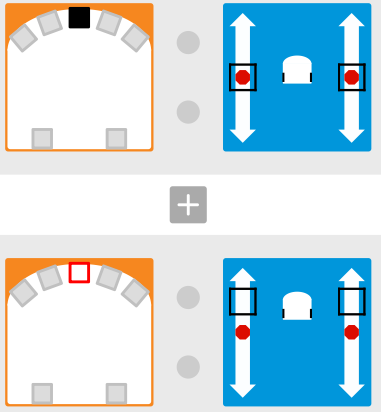
\includegraphics[width=.4\textwidth]{likes-forward}}
	\ffigbox
	{\caption{Ein Bulldozer mit Raupen}\label{fig.bull}}
	{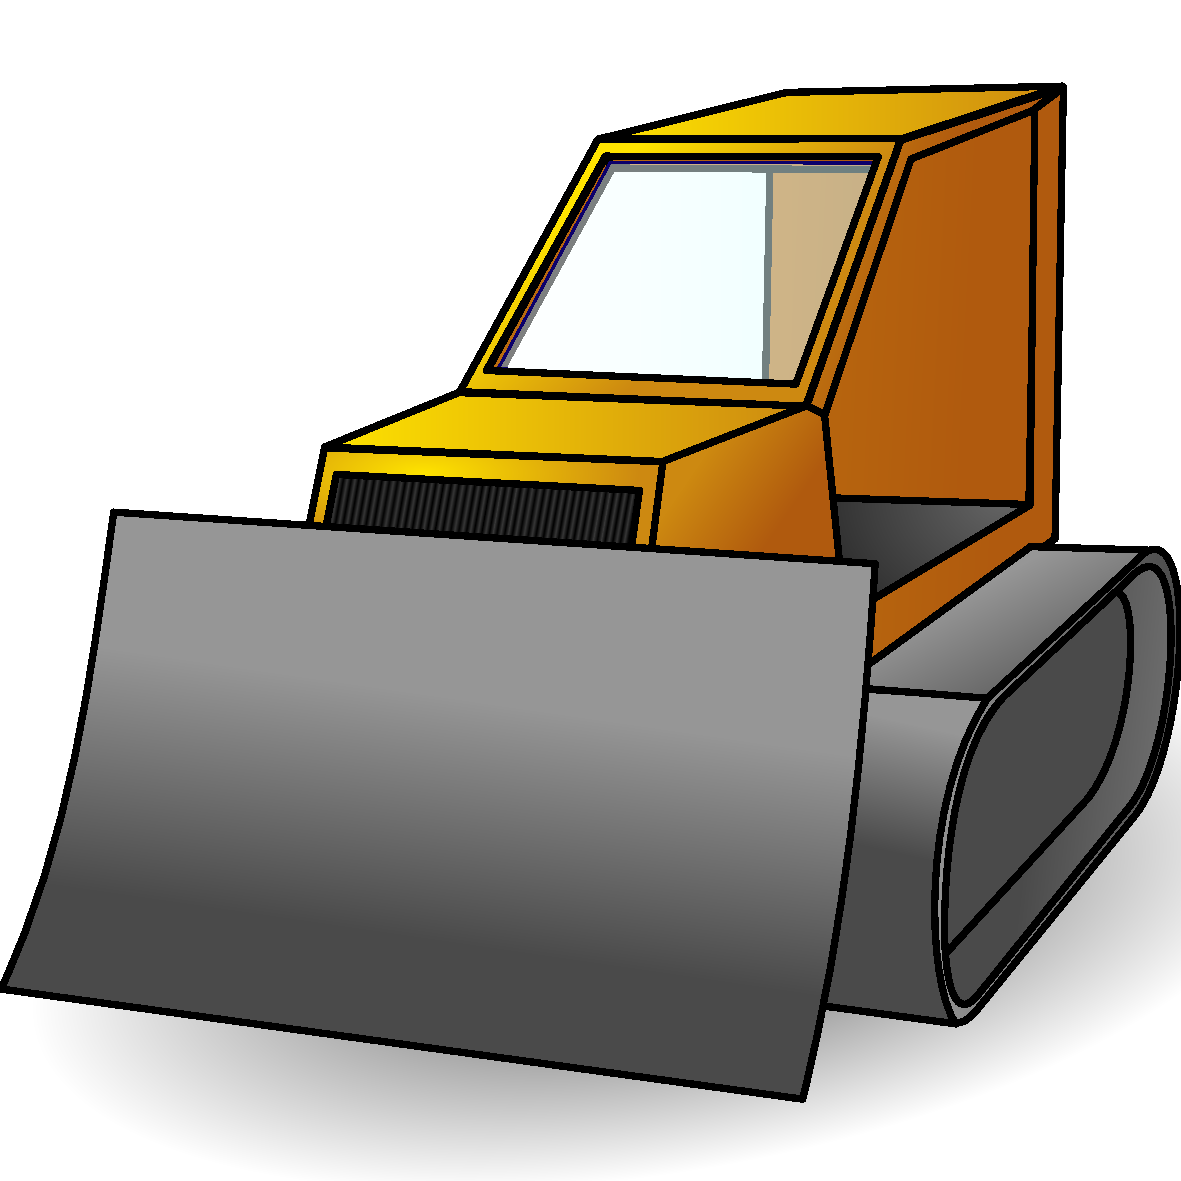
\includegraphics[width=.35\textwidth]{bulldozer}}
\end{floatrow}
\end{figure}

\sect{Steuerung des Roboter Thymio}

Der Roboter Thymio hat kein Steuerrad wie ein Auto und kein Lenker wie ein Fahrrad. Wie kann man ihn also lenken? Der Roboter benutzt ein \emph{Differentialgetriebe}, welches ähnlich funktioniert wie bei einem Raupenfahrzeug, z.B. einem Bulldozer (\cref{fig.bull}).
Die gewünschte Richtung wird mit Hilfe von \emph{unterschiedlichen} Geschwindigkeiten des linken und rechten Rades erreicht. Dreht das rechte Rad schneller als das linke, biegt das Fahrzeug nach links ab und dreht das linke Rad schneller als das rechte, biegt das Fahrzeug nach rechts ab.

In VPL wendet man das Differentialgetriebe an, indem man den linken und rechten Schieberegler des Motoraktionsblocks einzeln einstellt und dadurch die Geschwindigkeit der Räder verschieden einstellen kann.
Um einen möglichst grossen Unterschied der Geschwindigkeiten zu erreichen, lässt man die Räder in die entgegengesetzten Richtungen drehen. Tatsächlich dreht sich das Fahrzeug auf der Stelle, falls sich die Räder mit der genau \emph{gleichen} Geschwindigkeit in die entgegengesetzte Richtung bewegen.

Zum Beispiel wird im Aktionsblock \blksm{differential} der linke Regler auf schnelle Geschwindigkeit rückwärts und der rechte Regler auf schnelle Geschwindigkeit vorwärts eingestellt.  Als Resultat wird der Roboter eine enge Linkskurve vollführen, wie dies auf dem kleinen Bild des Roboter bzw. des Motoraktionsblocks dargestellt ist.

Experimentieren Sie mit einem Ereignis-Aktions-Paar wie diesem: \blkc{turning}

Stellen Sie den linken und rechten Schieber ein und lassen Sie das Programm laufen. Stoppen Sie dann den Roboter durch klicken auf \blksm{stop}. Ändern Sie nun die Schieberegler und versuchen Sie es erneut!

\trickbox{Das kleine Bild in der Mitte stellt den Thymio in seiner Bewegung dar. Wenn die Animation anhält, zeigt Thymio in die Richtung, in die sich der Roboter bewegen wird. }
	
\sect{Der Roboter mag Sie}

Ein echtes Haustier folgt seinem Meister. Damit der Roboter Ihrer Hand folgt,
muss man zwei weitere Ereignis-Aktions-Paare hinzufügen. Falls der Roboter ein Objekt vor seinem ganz links platzierten Distanzsensor wahrnimmt, soll er nach links drehen und falls er ein Objekt vor seinem ganz rechts platzierten Distanzsensor wahrnimmt, soll er nach rechts abbiegen.
                                                       
{\raggedleft \hfill Beispielprogramm \bu{likes.aesl}}

Das Programm für ''Der Roboter mag Sie'' besteht aus zwei Ereignis-Aktions-Paaren (\cref{fig.likes}).
Probieren Sie die Regler an jedem Motoraktionsblock aus!

\begin{figure}
	\subfigure[Der Roboter mag Sie]{
		\label{fig.likes}
		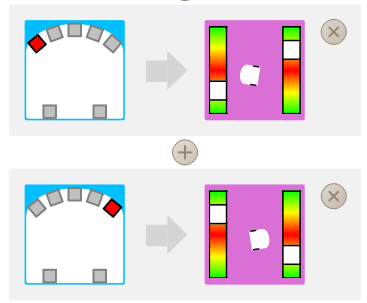
\includegraphics[width=.4\textwidth]{likes-turns}
	}
	\hfill
	\subfigure[Der Roboter mag Sie nicht]{
		\label{fig.hates}
		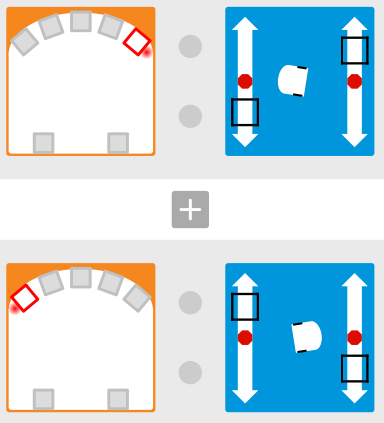
\includegraphics[width=.4\textwidth]{hates}
	}
	\caption{Programme für den Haustier-Roboter}\label{fig.likes-hates}
\end{figure}

\exercisebox{\thechapter.1}{Verändern Sie den Haustierroboter so, dass er vorwärts fährt, falls das Programm am laufen ist und stoppt, falls er das Ende des Tisches wahrnimmt.}

\exercisebox{\thechapter.2}{Was geschieht, wenn Sie die Reihenfolge der Ereignis-Aktions-Paare ändern?}

\sect{Der Roboter mag Sie nicht}

Manchmal mag dein Roboterhaustier in schlechter Laune sein und von deiner Hand zurückweichen. Erstellen Sie ein Programm, welches dieses Verhalten auslöst.

{\raggedleft \hfill Beispielprogramm \bu{does-not-like.aesl}}

Öffnen Sie das Programm für den Haustierroboter, der Sie mag und ändern Sie die Zusammenhänge zwischen Ereignissen und Aktionen. Das Erkennen eines Hindernisses beim linken Sensor bewirkt, dass der Roboter nach rechts abbiegt, 
während das Erkennen eines Hindernisses beim rechten Sensor bewirkt, 
dass der Roboter nach links abbiegt (\cref{fig.hates}).

% \begin{figure}[htb]
% \begin{center}
% \gr{hates}{0.4}
% \caption{The robot doesn't you}\label{fig.hates}
% \end{center}
% \end{figure}

\exercisebox{\thechapter.3} {Die vorderen horizontalen Sensoren sind von 0 bis 4 nummeriert (von links nach rechts). Die hinteren Sensoren tragen die Nummern 5 (links) und 6 (rechts). Ändern Sie das Programm \cref{fig.likes-hates} so dass anstelle der Sensoren 0 und 4...
\begin{itemize}[noitemsep,nosep,leftmargin=*]
\item die Sensoren 1 und 3 verwendet werden für die Drehung nach links bzw. rechts, 
\item die Sensoren 0 und 1 verwendet werden für die Linkskurve und die Sensoren 3 und 4 für die Rechtskurve.
\item Fügen Sie Ereignis-Aktions-Paare hinzu für die Sensoren 5 und 6.
\end{itemize}
}

\bigskip

\trickbox{\cref{a.tech} erklärt, wie man die Schieber für die Motorengeschwindigkeit präzise steuern kann.}

\informationbox{Sensoren im Fortgeschrittenen-Modus}{Im Fortgeschrittenen-Modus (siehe \cref{ch.time}), gibt es eine zusätzliche Art, um die Ereignisse abhängig von den Sensoren auszulösen (nachzulesen in  \cref{a.tech}).}
